\subsection{Démarrer les différents services Hadoop:}

\begin{enumerate}
\item \textbf{Démarrage des services Hbase: } Tout d'abord s'assurer que les services Hadoop sont en marche.

\item Pour démarrer HBase, exécutez la commande ci-dessous à partir du dossier bin : \textit{start-hbase.cmd}
\begin{figure}[h]
	\centering
    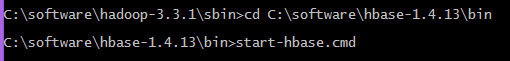
\includegraphics[scale=0.6]{img/part3/3.6}
    \caption{Démarrage des services HBase}
\end{figure}

\newpage
cette fenêtre d'invite de commande s'ouvrira comme suit :
\begin{figure}[h]
	\centering
    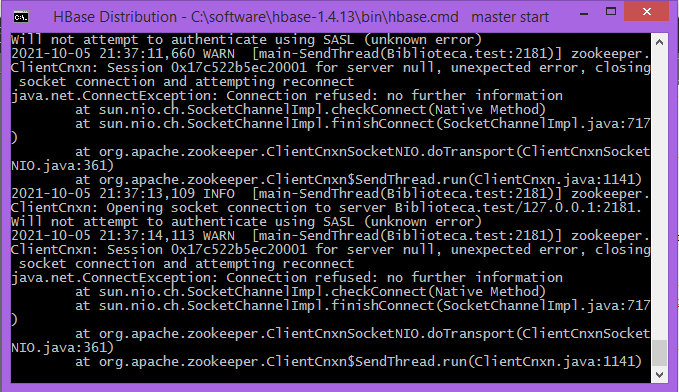
\includegraphics[scale=0.6]{img/part3/3.7}
    \caption{Fenêtres d'invite de commande HBase}
\end{figure}

\item on finit par le démarrage du service Rest de hBase avec la commande \texttt{hbase rest start}
\begin{figure}[h]
	\centering
    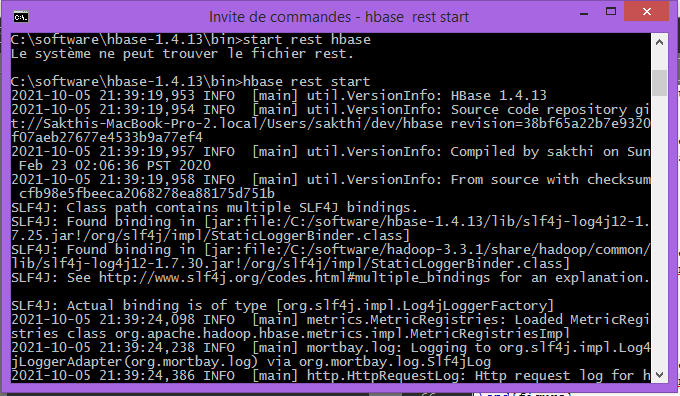
\includegraphics[scale=0.6]{img/part3/3.8}
    \caption{Fenêtres d'invite de commande Du serviceRrest HBase}
\end{figure}

\end{enumerate}